\chapter{PHASE III - IDMC et analyses intérimaires}

\section{Idée générale}
Un essai clinique de phase III dure souvent plusieurs années, on a donc la nécessité de s’assurer que « tout va bien » pendant l’essai.
\begin{figure}[H]
    \centering
    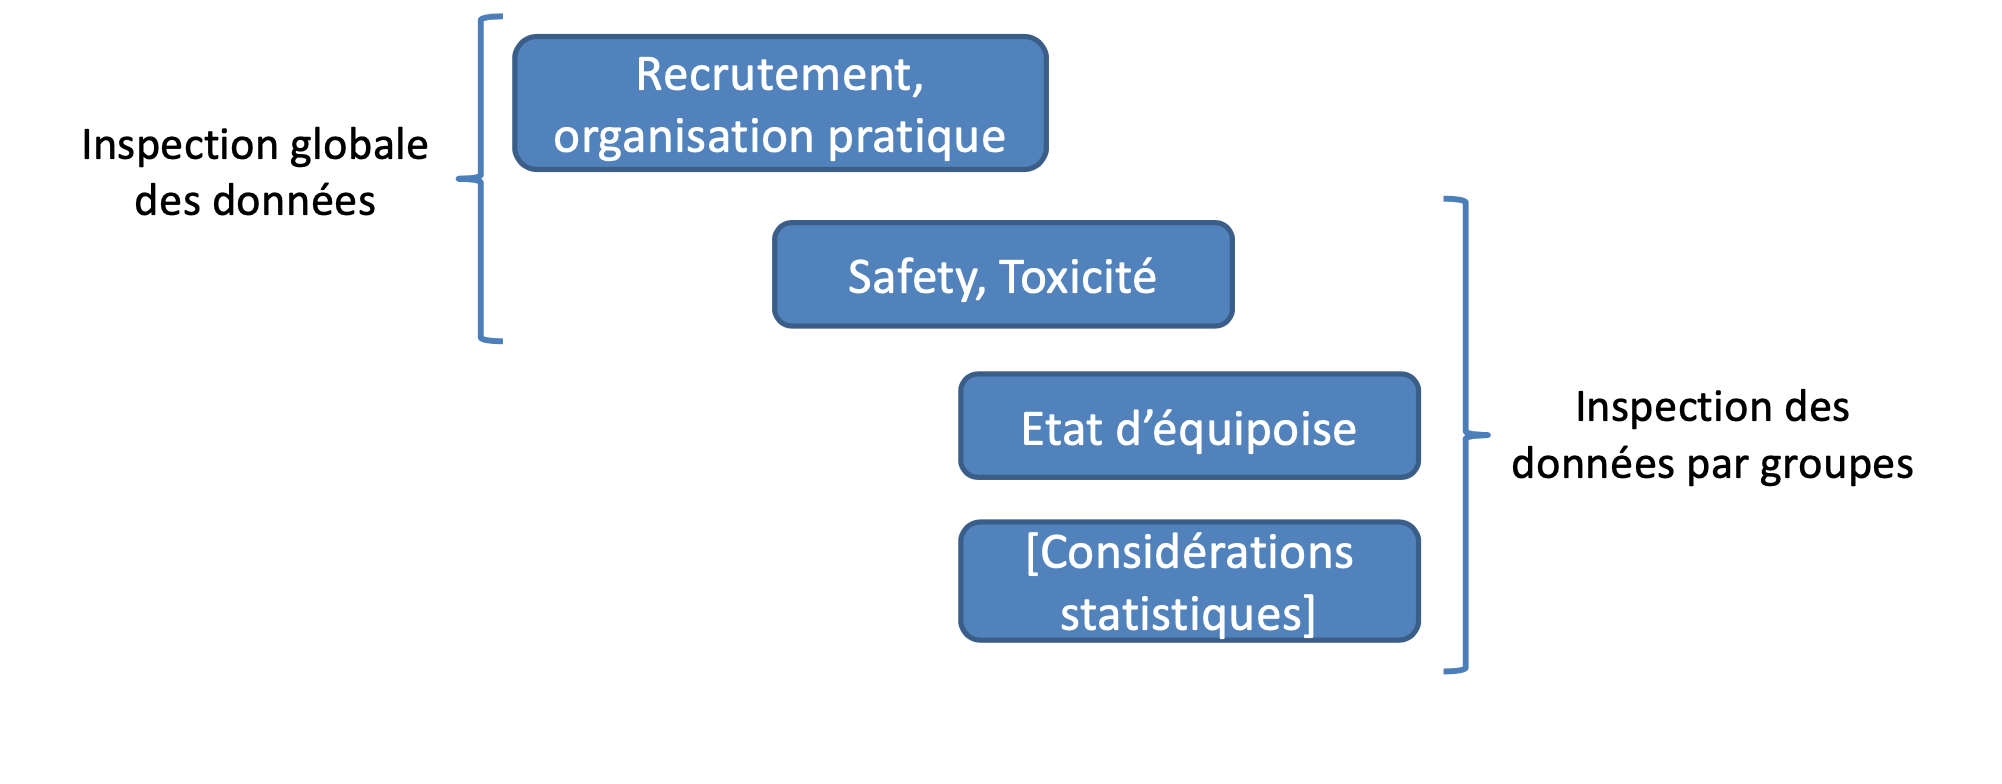
\includegraphics[scale = 0.4]{images/IDMC.png}
    \caption{IDMC: idée générale}
    \label{fig:IDMC}
\end{figure}
Sauf qu'inspecter(régulièrement) les données par groupe est problématique pour différentes raisons :
\begin{itemize}
    \item Problèmes avec l’aveugle
\item Risque de sur-interprétation des résultats et de démotivation
pour l’essai en cours
\item Risque de suspicion de fraude (si des actions sont/doivent être prises)
\item Problème de méthodologie statistique (tests multiples).
\end{itemize}

\vspace{0.5cm}

\begin{center}
    $\Rightarrow$ Independent Data Monitoring Committee (IDMC)
\end{center}
\section{IDMC}


\section{Analyses intérimaires}

\begin{itemize}
    \item Toute une série de points n’ont pas d’impact sur la méthodologie statistique de l’essai :
    \begin{itemize}
        \item Monitoring des données individuelles des patients
\item Monitoring du recrutement, des centres actifs, de la participation des
investigateurs, etc
\item Monitoring des aspects logistique (approvisionnement en médicaments, encodage des données, etc)
\item Monitoring global de la safety/toxicité des patients sans comparaison formelle par groupe
    \end{itemize}
\item Par contre, réaliser une comparaison formelle des bras de traitement requiert une méthodologie adaptée !
– Contrôle du risque d’erreur de type I
\end{itemize}
\subsection{Problème de multiplicité}
On sait que le risque global d’erreur de type I augmente (très rapidement) avec le nombre de comparaisons.

\subsection{Analyses intérimaires : Comment contrôler le risque d’erreur de type I global}

L'idée est de diviser le $\alpha$ sur les différents tests réalisés(et prendre en compte la corrélation entre les statistiques de tests successives).

